\chapter{Progettazione concettuale}
    \section{Class Diagram del dominio del problema}

    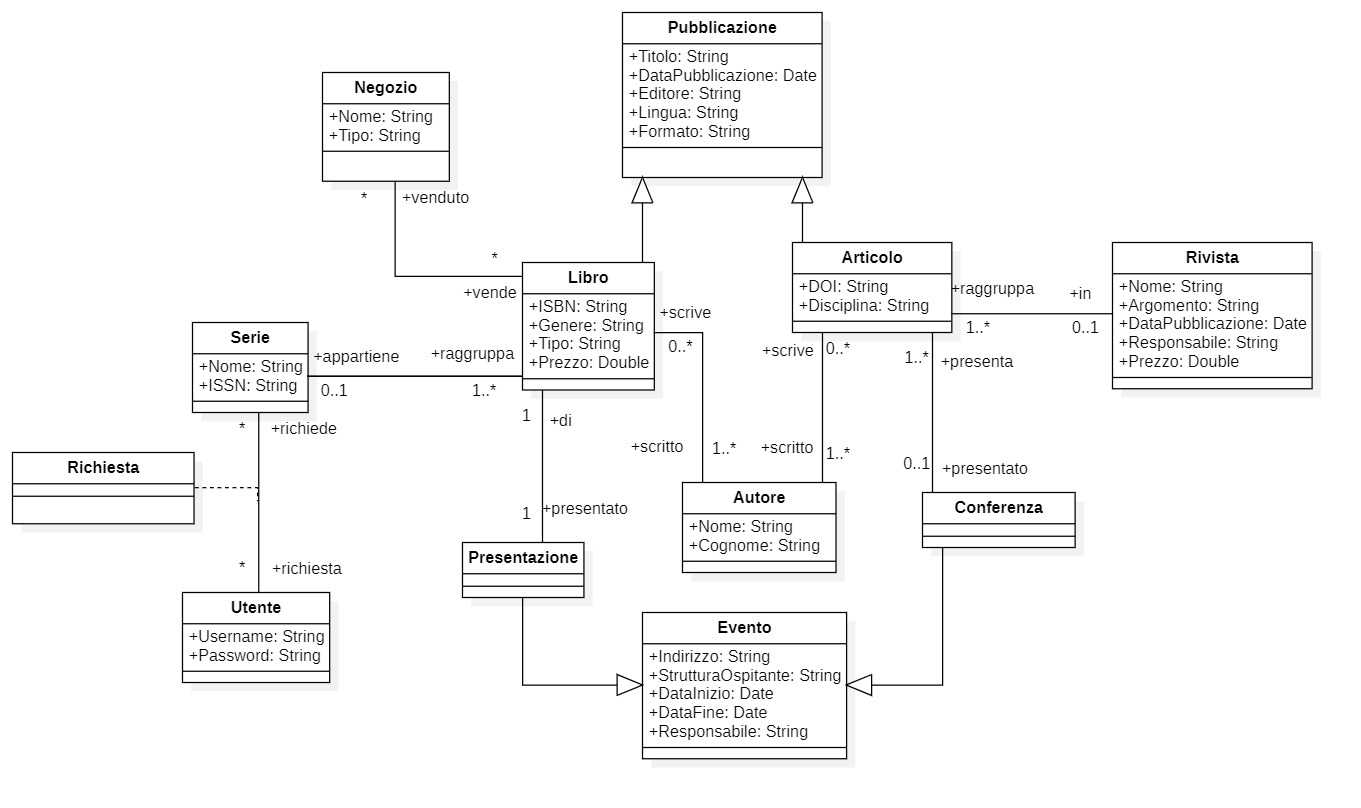
\includegraphics[scale=0.25, center]{Immagini/CD_dominio_del_problema.png}
        
    \section{Dizionario delle classi}

    \begin{longtable}[c]{|l|l|}
        \hline
        \textbf{Classe} &
          \textbf{Attributi} \\ \hline
        \endfirsthead
        %
        \endhead
        %
        Articolo &
          \begin{tabular}[c]{@{}l@{}}Titolo (String): Titolo di un articolo scientifico.\\ Autori (String): Stringa contenente il/gli autore/i di\\ un articolo.\\ Editore (String): Casa editrice dell'articolo.\\ Disciplina (String): Disciplina approfondita dall'articolo.\\ Formato (String): Formato dell'articolo (Cartaceo, Digitale\\ o Audiolibro).\\ DOI (String): Identificativo di un oggetto digitale.\\ Lingua (String): Lingua in cui è scritto l'articolo\end{tabular} \\ \hline
        Autore &
          \begin{tabular}[c]{@{}l@{}}Nome (String): Nome dell'autore.\\ Cognome (String): Cognome dell'autore.\end{tabular} \\ \hline
        Conferenza &
          \begin{tabular}[c]{@{}l@{}}Nome (String): Nome dell'evento che ospita la conferenza.\\ Responsabile (String): Nome e cognome del responsabile\\ della conferenza.\\ StrutturaOspitante (String): Nome della struttura che ospita\\ la conferenza.\\ Indirizzo (String): Indirizzo dell'evento.\\ DataInizio (Date): Data in cui inizia l'evento.\\ DataFine (Date): Data in cui finisce l'evento.\end{tabular} \\ \hline
        Libro &
          \begin{tabular}[c]{@{}l@{}}Titolo (String): Titolo di un libro.\\ Autori (ArrayList\textless{}Autore\textgreater{}): ArrayList che contiene gli\\ autori (o l'autore) di un libro\\ Genere (String): Genere di un libro.\\ Editore (String): Casa editrice di un libro.\\ DataPubblicazione (Date): Data di pubblicazione di un\\ libro.\\ ISBN (String): Codice identificativo di un libro.\\ Formato (String): Formato di un libro.\\ Lingua (String): Lingua in cui un libro è scritto.\\ Prezzo (Double): Prezzo di vendita di un libro.\\ SerieDiAppartenenza (String): Nome della serie a cui\\ appartiene un libro.\\ ISSNSerieDiAppartenenza (String): Identificativo della\\ serie a cui appartiene un libro.\end{tabular} \\ \hline
        Utente &
          \begin{tabular}[c]{@{}l@{}}Username (String): Nome di un utente.\\ Password (String): Password di un utente.\\ Permessi (Int): Livello di permessi di un utente.\end{tabular} \\ \hline
        \end{longtable}
        
    \section{Dizionario delle associazioni}